\section{Bucket sort}
\label{sec:bucket_sort}

\begin{frame}
	\frametitle{Sorting exams: Bucket Sort}
	\framesubtitle{Some Saturdays look like this...}
	\begin{center}
		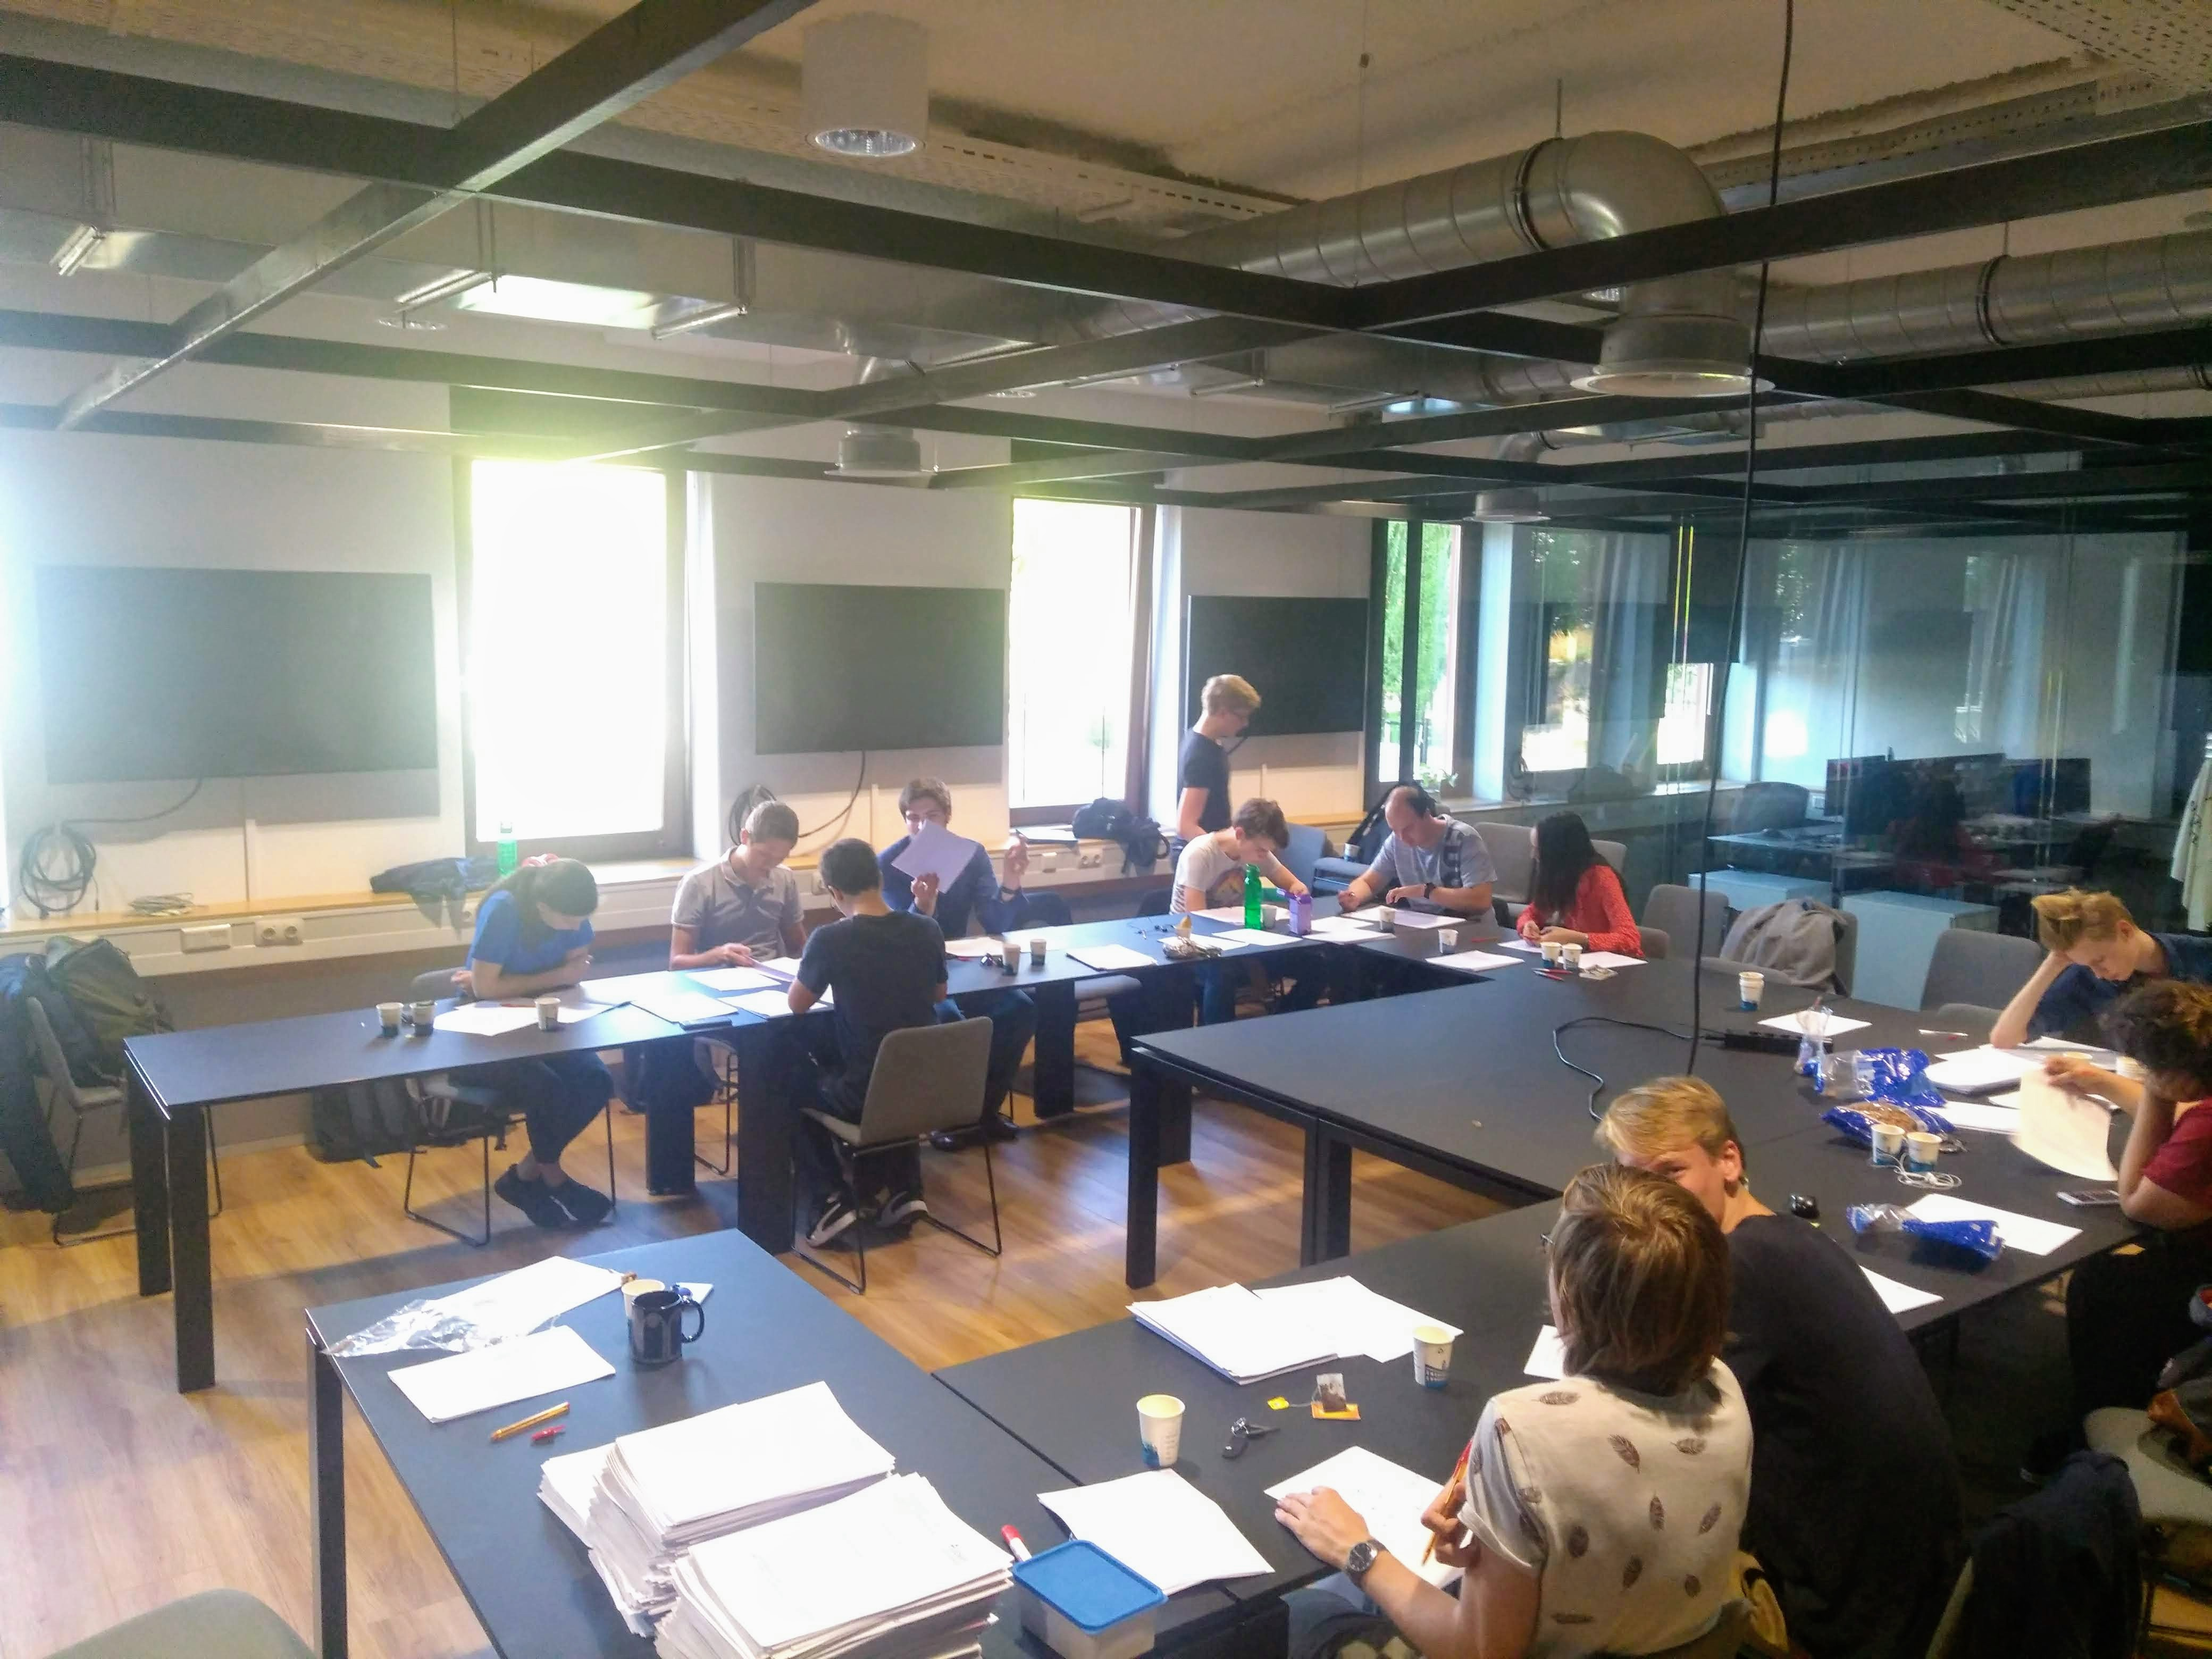
\includegraphics[trim={0 0 0 35cm}, clip, width=0.9\textwidth]{figures/grading.jpg}\\
		\hspace*{15pt}\hbox{\scriptsize Image By:\thinspace{\itshape Stefan Hugtenburg}}
	\end{center}
\end{frame}

\begin{frame}
	\frametitle{Bucket Sort}
	\framesubtitle{The Stephen Tatlock algorithm\dots \only<3->{\tiny Okay that was probably too obscure a reference}}

		\begin{block}{Bucket Sort}
			\begin{enumerate}
				\item Sort the items into buckets (e.g. based on first letter of last name).
					\pause
				\item Sort every bucket.
					\pause
				\item Concatenate all buckets together.
			\end{enumerate}
		\end{block}	
		\pause
		\vspace{-0.2cm}
		\begin{questionblock}{Why is this good?}
			Why should we use this?
		\end{questionblock}
		\pause
		\vspace{-0.2cm}
		\begin{answerblock}{Well...}
			\begin{itemize}
				\item Great for parallelisation!
				\item Great for humans (sorting a bucket can be done using a different algorithm, everyone can pick their own
					favourite).
				\item Average case analysis is interesting for this algorithm (and gets us to something close to linear time for
					average case).
			\end{itemize}
		\end{answerblock}
\end{frame}


